%!TEX root = ../dokumentation.tex
\section{ERM allink.planer}
Als Ausgangslage dient mir das ERM des allink.planer. Die Entitäten Person und Project werden mit dem Wochenplaner verknüpft.

\begin{figure}[!ht]
\begin{center}
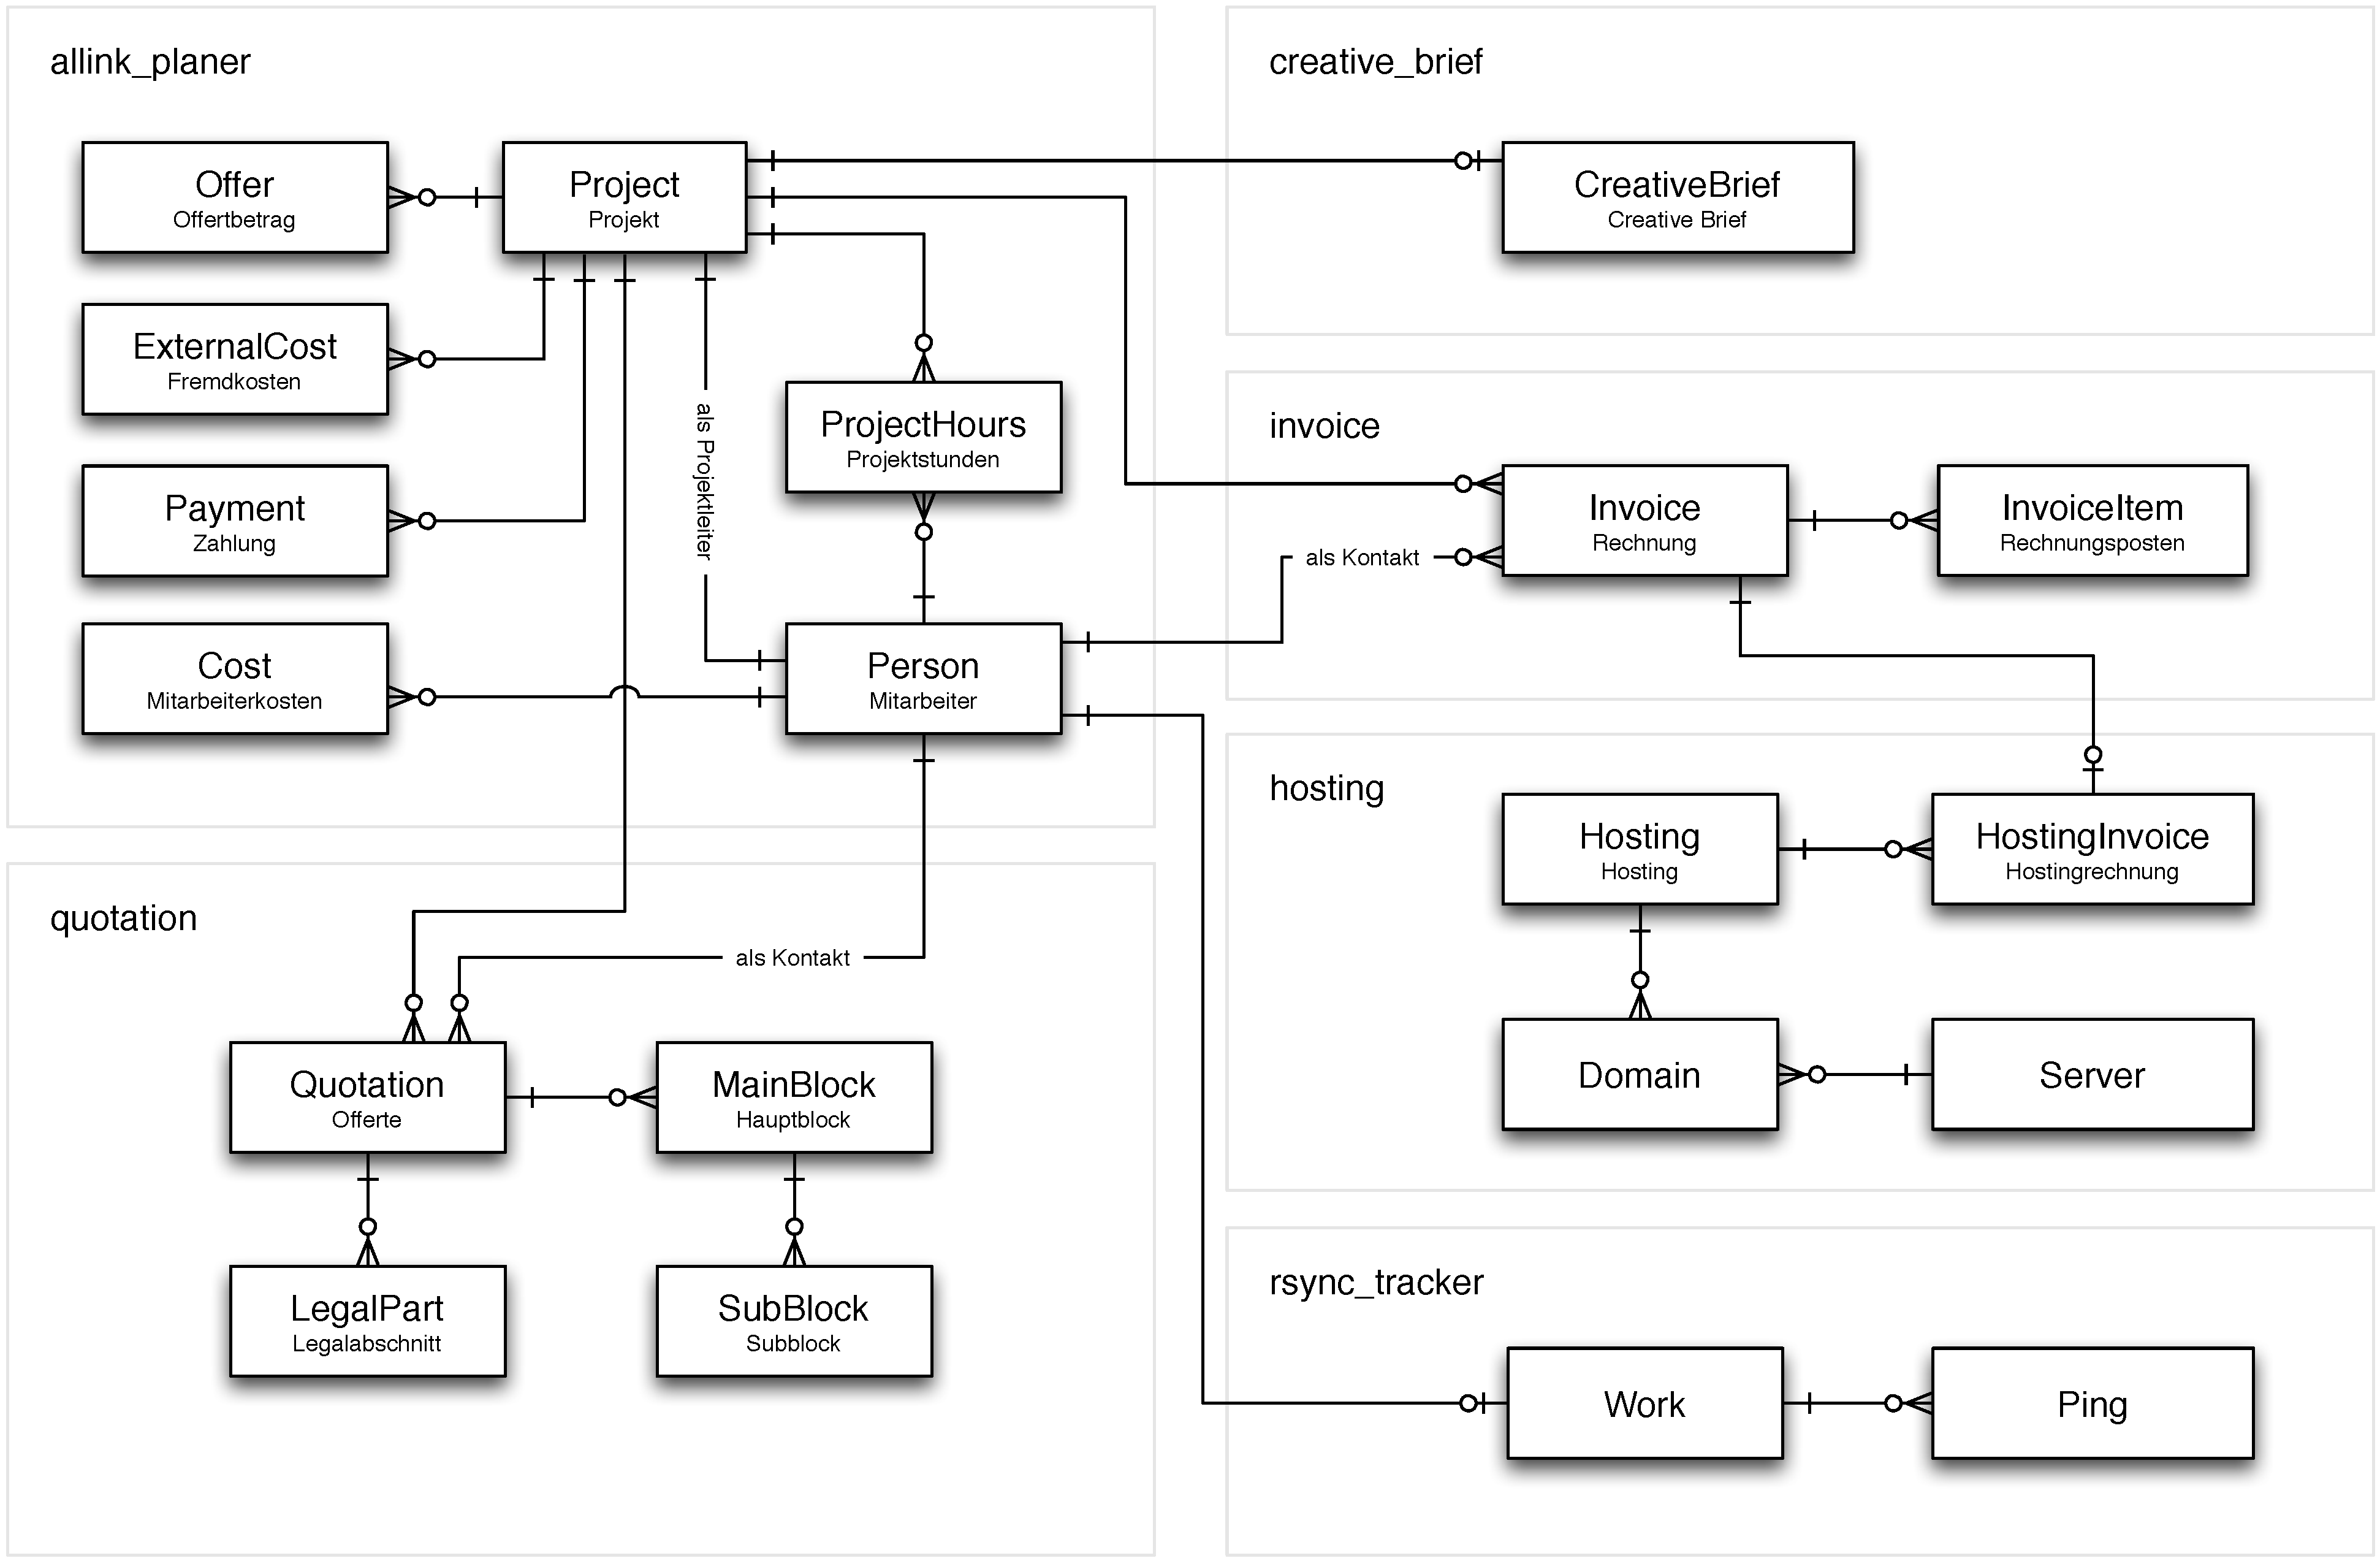
\includegraphics[width=0.99\textwidth,angle=0]{./bilder/erm_planer.pdf}
\caption{ERM allink.planer}
\end{center}
\end{figure}
\footnotetext{Entommen aus allink.planer}

\clearpage

\section{ERM Wochenplaner}
\begin{figure}[!ht]
\begin{center}
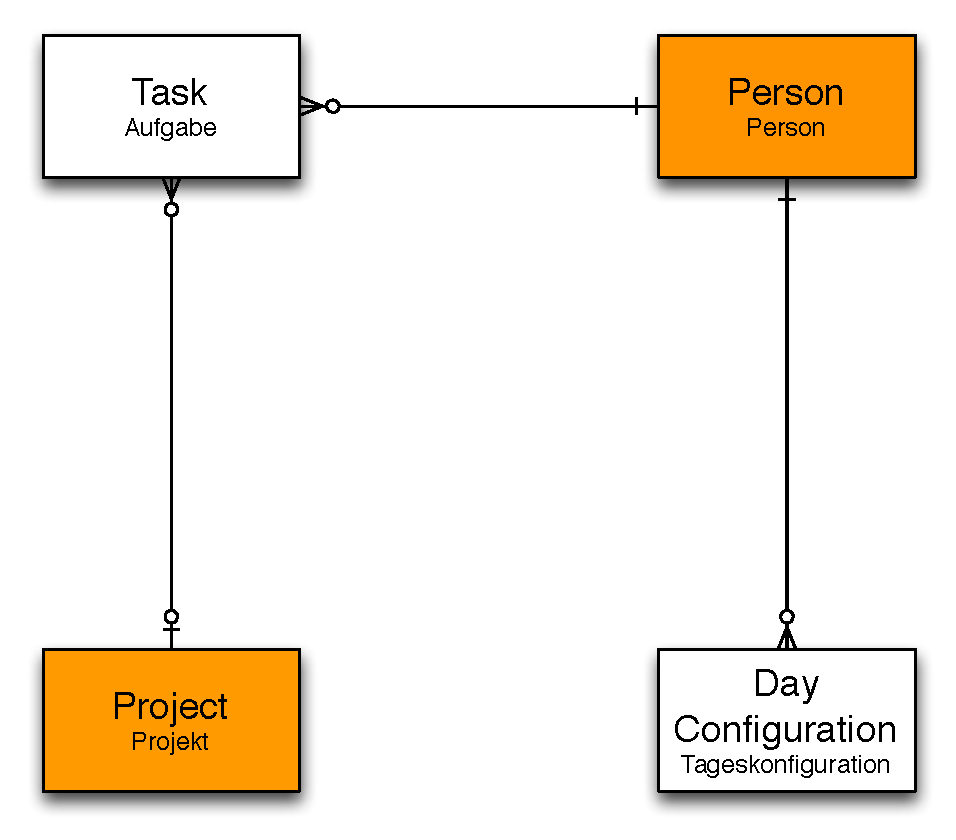
\includegraphics[width=0.99\textwidth,angle=0]{./bilder/erm.pdf}
\caption{ERM Wochenplaner (die Orange hinterlegten Entitäten stammen aus dem allink.planer)}
\end{center}
\end{figure}
\footnotetext{Eigene Darstellung}

\section{Design}
\subsection{Altes Design}
\begin{figure}[!ht]
\begin{center}
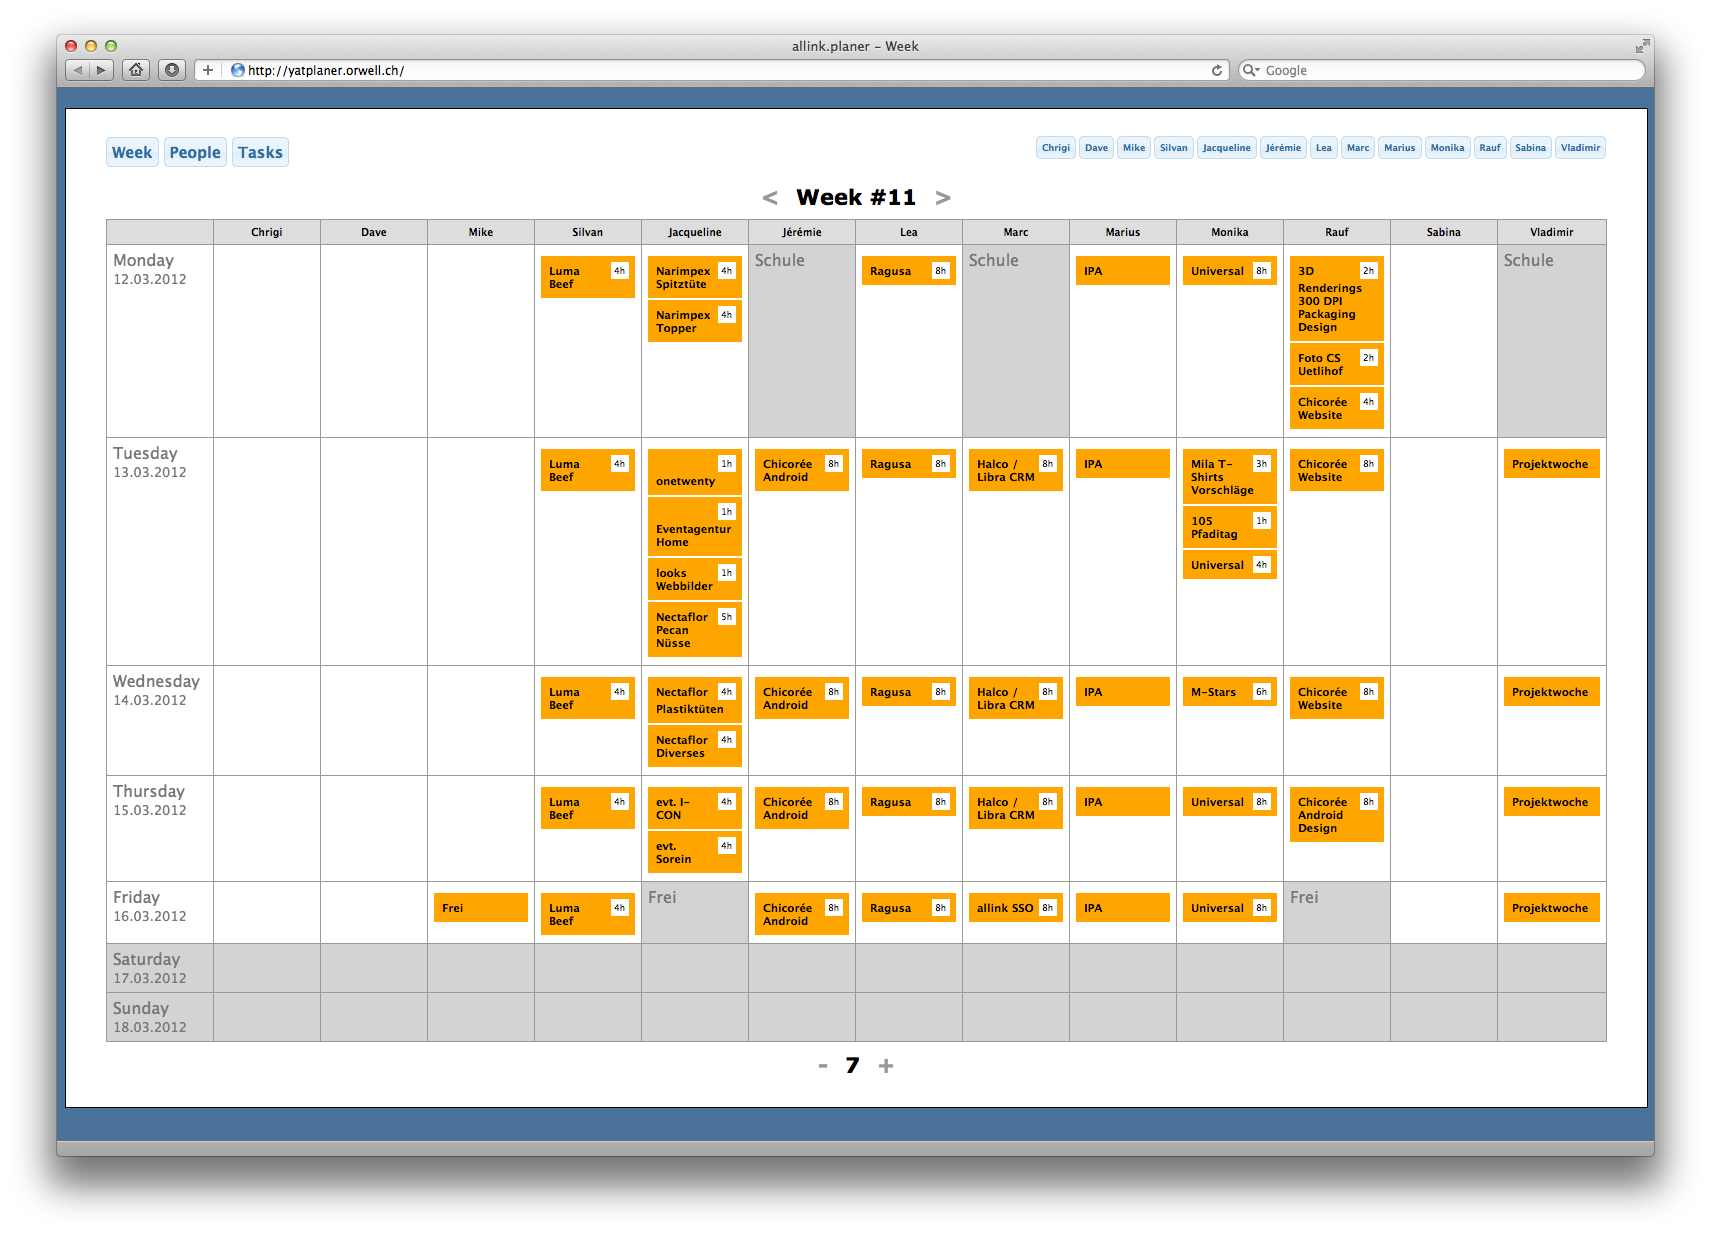
\includegraphics[width=0.99\textwidth,angle=0]{./bilder/yatplaner.png}
\caption{Bisheriges Design des yatplaner}
\end{center}
\end{figure}

\clearpage
\section{Neues Design}
\begin{figure}[!ht]
\begin{center}
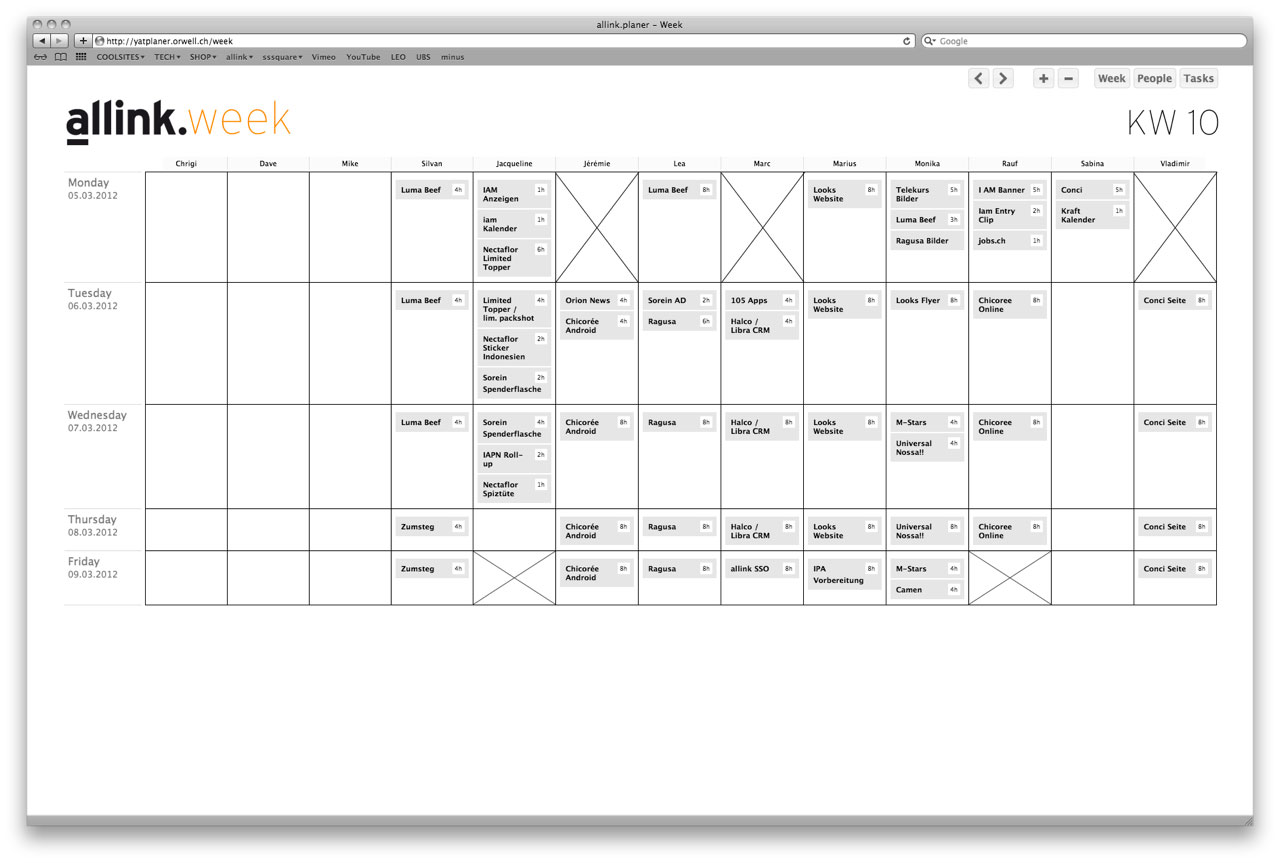
\includegraphics[width=0.99\textwidth,angle=0]{./bilder/wochenplaner.jpg}
\caption{Neues Design}
\end{center}
\end{figure}

%\section{System-Beschreibung}

\section{Modellierung (Django, aufsetzen Projekt)/Backend }
Über das Django-Framework kann man die Modelle der Klassen bzw. auch Entitäten erfassen.
Alle Modelle können als Applikationen über einen Administratorbereich durch CRUD gesteuert werden.
\section{Layout}
Das Layout bleibt, bis auf einige kleine Anpassungen, dasselbe.
\section{Effektive Umsetzung der Applikation}
Modelle erzeugt\\
urls für wochenplaner
Adminbereich eingerichte, App lebt im admin und muss von dort aus gesteuert werden\\
\section{Templating Wochenansicht/Frontend}
Template für Wochenansicht erstellt
Daten werden an template übergeben
Tage werden korrekt ausgeben
Tasks sind an der richtigen Stelle (Tag und Person)
\section{JS Funktionalität (CRUD mit jQueryUI \& AJAX) }
Die Wochenansicht der Tasks ist eine rein statische Ansicht.
Alle Tasks und Sperrtage können über den Django admin per CRUD gesteuert werden. Dies ist aber nur ein Teil der bestehenden Funktionalität.
Es wird eine CRUD-Funktionalität im Frontend benötigt. Diese werde ich mit jQueryUI möglich machen da ich mit jQuery am meisten Erfahrung habe.
Sich in Alternativen einzuarbeiten benötigt zu viel Zeit und ist nicht mit jQuery kompatibel.
Per jQueryUI können alle Task frei verschoben werden zu jedem Tag und/oder Person.
Per AJAX werden neue Tasks automatisch in die DB geschrieben und danach ins HTML eingefügt.
\section{Implementierung}
\section{Erreichte Ziele}
